% Options for packages loaded elsewhere
% Options for packages loaded elsewhere
\PassOptionsToPackage{unicode}{hyperref}
\PassOptionsToPackage{hyphens}{url}
%
\documentclass[
  ignorenonframetext,
  aspectratio=169,
  handout]{beamer}
\newif\ifbibliography
\usepackage{pgfpages}
\setbeamertemplate{caption}[numbered]
\setbeamertemplate{caption label separator}{: }
\setbeamercolor{caption name}{fg=normal text.fg}
\beamertemplatenavigationsymbolsempty
% remove section numbering
\setbeamertemplate{part page}{
  \centering
  \begin{beamercolorbox}[sep=16pt,center]{part title}
    \usebeamerfont{part title}\insertpart\par
  \end{beamercolorbox}
}
\setbeamertemplate{section page}{
  \centering
  \begin{beamercolorbox}[sep=12pt,center]{section title}
    \usebeamerfont{section title}\insertsection\par
  \end{beamercolorbox}
}
\setbeamertemplate{subsection page}{
  \centering
  \begin{beamercolorbox}[sep=8pt,center]{subsection title}
    \usebeamerfont{subsection title}\insertsubsection\par
  \end{beamercolorbox}
}
% Prevent slide breaks in the middle of a paragraph
\widowpenalties 1 10000
\raggedbottom
\AtBeginPart{
  \frame{\partpage}
}
\AtBeginSection{
  \ifbibliography
  \else
    \frame{\sectionpage}
  \fi
}
\AtBeginSubsection{
  \frame{\subsectionpage}
}
\usepackage{iftex}
\ifPDFTeX
  \usepackage[T1]{fontenc}
  \usepackage[utf8]{inputenc}
  \usepackage{textcomp} % provide euro and other symbols
\else % if luatex or xetex
  \usepackage{unicode-math} % this also loads fontspec
  \defaultfontfeatures{Scale=MatchLowercase}
  \defaultfontfeatures[\rmfamily]{Ligatures=TeX,Scale=1}
\fi
\usepackage{lmodern}

\ifPDFTeX\else
  % xetex/luatex font selection
\fi
% Use upquote if available, for straight quotes in verbatim environments
\IfFileExists{upquote.sty}{\usepackage{upquote}}{}
\IfFileExists{microtype.sty}{% use microtype if available
  \usepackage[]{microtype}
  \UseMicrotypeSet[protrusion]{basicmath} % disable protrusion for tt fonts
}{}
\makeatletter
\@ifundefined{KOMAClassName}{% if non-KOMA class
  \IfFileExists{parskip.sty}{%
    \usepackage{parskip}
  }{% else
    \setlength{\parindent}{0pt}
    \setlength{\parskip}{6pt plus 2pt minus 1pt}}
}{% if KOMA class
  \KOMAoptions{parskip=half}}
\makeatother


\usepackage{longtable,booktabs,array}
\newcounter{none} % for unnumbered tables
\usepackage{calc} % for calculating minipage widths
\usepackage{caption}
% Make caption package work with longtable
\makeatletter
\def\fnum@table{\tablename~\thetable}
\makeatother
\usepackage{graphicx}
\makeatletter
\newsavebox\pandoc@box
\newcommand*\pandocbounded[1]{% scales image to fit in text height/width
  \sbox\pandoc@box{#1}%
  \Gscale@div\@tempa{\textheight}{\dimexpr\ht\pandoc@box+\dp\pandoc@box\relax}%
  \Gscale@div\@tempb{\linewidth}{\wd\pandoc@box}%
  \ifdim\@tempb\p@<\@tempa\p@\let\@tempa\@tempb\fi% select the smaller of both
  \ifdim\@tempa\p@<\p@\scalebox{\@tempa}{\usebox\pandoc@box}%
  \else\usebox{\pandoc@box}%
  \fi%
}
% Set default figure placement to htbp
\def\fps@figure{htbp}
\makeatother





\setlength{\emergencystretch}{3em} % prevent overfull lines

\providecommand{\tightlist}{%
  \setlength{\itemsep}{0pt}\setlength{\parskip}{0pt}}



 


\makeatletter
\@ifpackageloaded{caption}{}{\usepackage{caption}}
\AtBeginDocument{%
\ifdefined\contentsname
  \renewcommand*\contentsname{Table of contents}
\else
  \newcommand\contentsname{Table of contents}
\fi
\ifdefined\listfigurename
  \renewcommand*\listfigurename{List of Figures}
\else
  \newcommand\listfigurename{List of Figures}
\fi
\ifdefined\listtablename
  \renewcommand*\listtablename{List of Tables}
\else
  \newcommand\listtablename{List of Tables}
\fi
\ifdefined\figurename
  \renewcommand*\figurename{Figure}
\else
  \newcommand\figurename{Figure}
\fi
\ifdefined\tablename
  \renewcommand*\tablename{Table}
\else
  \newcommand\tablename{Table}
\fi
}
\@ifpackageloaded{float}{}{\usepackage{float}}
\floatstyle{ruled}
\@ifundefined{c@chapter}{\newfloat{codelisting}{h}{lop}}{\newfloat{codelisting}{h}{lop}[chapter]}
\floatname{codelisting}{Listing}
\newcommand*\listoflistings{\listof{codelisting}{List of Listings}}
\makeatother
\makeatletter
\makeatother
\makeatletter
\@ifpackageloaded{caption}{}{\usepackage{caption}}
\@ifpackageloaded{subcaption}{}{\usepackage{subcaption}}
\makeatother

\usepackage{bookmark}
\IfFileExists{xurl.sty}{\usepackage{xurl}}{} % add URL line breaks if available
\urlstyle{same}
\hypersetup{
  pdftitle={Waves},
  pdfauthor={Davit Potoyan},
  hidelinks,
  pdfcreator={LaTeX via pandoc}}


\title{\texorpdfstring{Waves}{Waves}}
\subtitle{\texorpdfstring{Chem 3240 · Lecture
2.1}{Chem 3240 · Lecture 2.1}}
\author{Davit Potoyan}
\date{}

\begin{document}
\frame{\titlepage}


\begin{frame}
\begin{block}{What is a wave?}
\protect\phantomsection\label{what-is-a-wave}
\begin{itemize}
\tightlist
\item
  A \textbf{wave} is a self-propagating \textbf{disturbance}
\item
  Transfers \textbf{energy, momentum, information}
\item
  Does \textbf{not} transport matter
\item
  Governed by the \textbf{wave equation}, a PDE
\end{itemize}

Two key families: \textbf{traveling waves} (propagate) and
\textbf{standing waves} (oscillate in place)
\end{block}

\begin{block}{Kinds of waves}
\protect\phantomsection\label{kinds-of-waves}
\begin{columns}[T]
\begin{column}{0.5\linewidth}
\includegraphics[width=0.9\linewidth,height=\textheight,keepaspectratio]{../../ch02/images/propage_stand.gif}
\end{column}

\begin{column}{0.5\linewidth}
\begin{itemize}
\tightlist
\item
  \textbf{Medium disturbance}: sound, strings, water
\item
  \textbf{Quantum waves}: complex wavefunctions for electrons, atoms
\item
  \textbf{Electromagnetic waves}: need \textbf{no medium}, travel in
  vacuum
\item
  \textbf{Gravitational waves}: ripples in spacetime
\end{itemize}
\end{column}
\end{columns}
\end{block}

\begin{block}{Transverse vs longitudinal}
\protect\phantomsection\label{transverse-vs-longitudinal}
\begin{columns}[T]
\begin{column}{0.5\linewidth}
\includegraphics[width=0.9\linewidth,height=\textheight,keepaspectratio]{../../ch02/images/ext_transverse_longitudinal.gif}
\end{column}

\begin{column}{0.5\linewidth}
\begin{itemize}
\tightlist
\item
  \textbf{Transverse}: disturbance is \textbf{perpendicular} to
  propagation
\item
  \textbf{Longitudinal}: disturbance is \textbf{along} propagation
\end{itemize}
\end{column}
\end{columns}
\end{block}

\begin{block}{Defining a wave mathematically}
\protect\phantomsection\label{defining-a-wave-mathematically}
\begin{itemize}
\tightlist
\item
  A disturbance \(u\) depends on space and time: \(u = f(x, t)\)
\item
  A surfer riding the wave sees it frozen at \(x'\)
\item
  A shore observer sees the front move: \(x = x' + vt\)
\end{itemize}

A right-moving wave of fixed shape:

\[u(x,t) = f(x-vt)\]

Set the front constant: \(x - vt = const \Rightarrow x = vt + const\)
(moves right). The form \(f(x+vt)\) moves \textbf{left}.
\end{block}

\begin{block}{Periodic traveling waves}
\protect\phantomsection\label{periodic-traveling-waves}
\begin{columns}[T]
\begin{column}{0.5\linewidth}
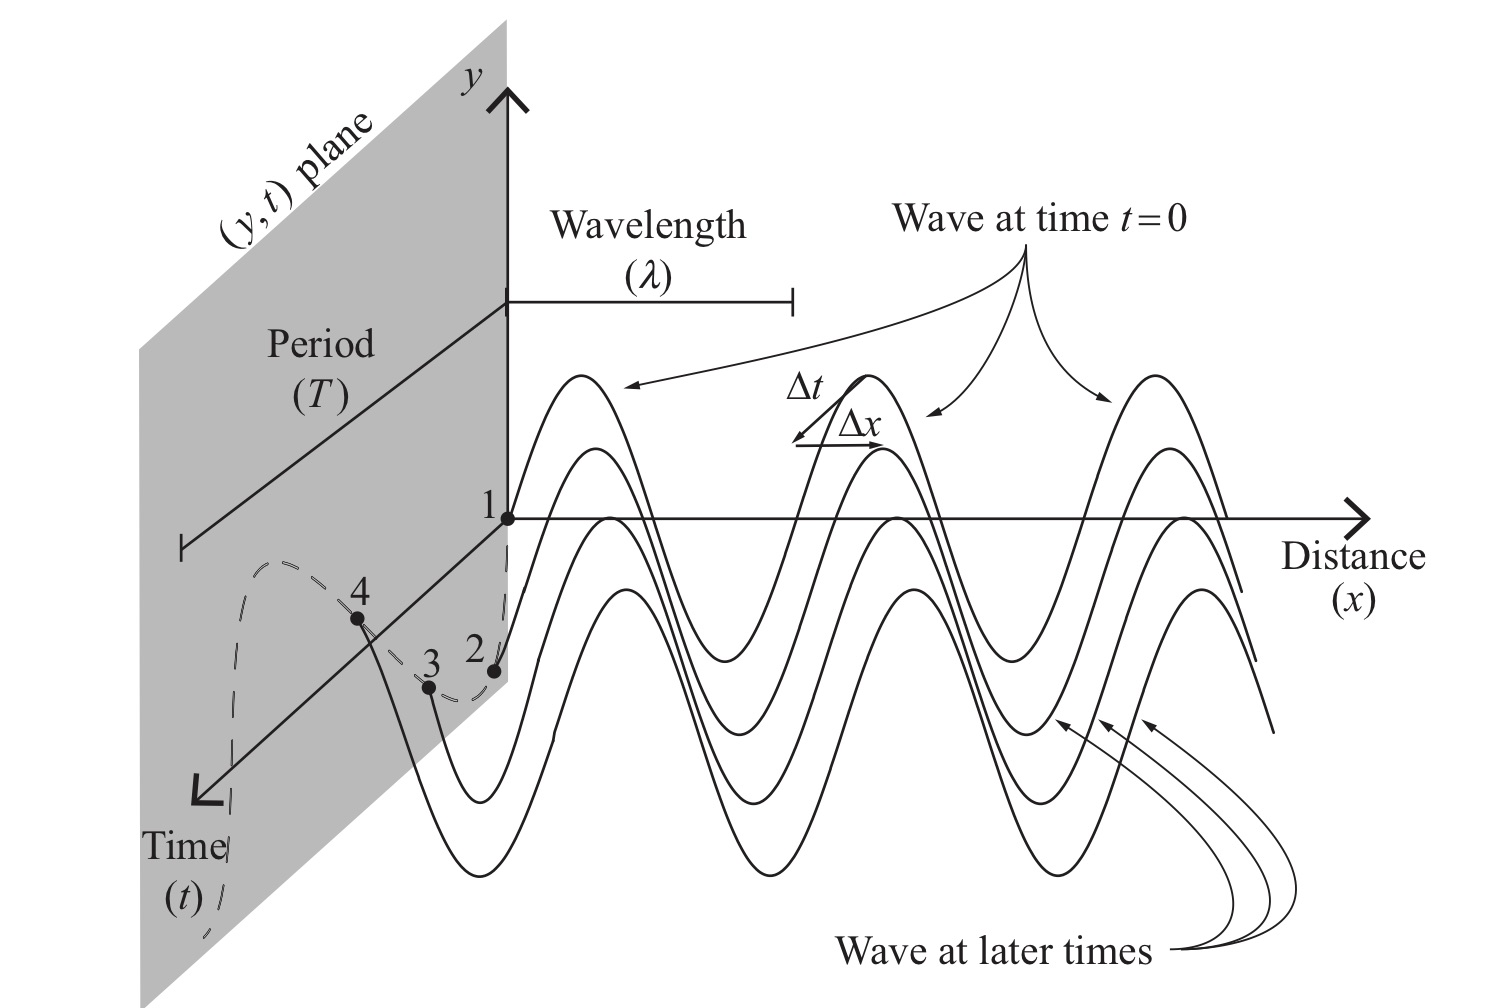
\includegraphics[width=0.9\linewidth,height=\textheight,keepaspectratio]{../../ch02/images/lec5_Introwave.jpg}
\end{column}

\begin{column}{0.5\linewidth}
A sine wave traveling along \(x\):

\[y(x,t)= A \sin(kx-\omega t+\phi)\]

\begin{itemize}
\tightlist
\item
  \textbf{Amplitude} \(A\): max disturbance
\item
  \textbf{Wave number} \(k\): periodicity in space
\item
  \textbf{Angular frequency} \(\omega = kv\): periodicity in time
\item
  \textbf{Phase} \(\phi\): starting point
\end{itemize}
\end{column}
\end{columns}
\end{block}

\begin{block}{Complex representation}
\protect\phantomsection\label{complex-representation}
\begin{itemize}
\tightlist
\item
  Easier to compute with \textbf{complex exponentials}, take real or
  imaginary part at the end
\end{itemize}

\[u(x,t) = Ae^{i(kx-\omega t)}\]

\begin{columns}[T]
\begin{column}{0.4\linewidth}
\includegraphics[width=0.8\linewidth,height=\textheight,keepaspectratio]{../../ch02/images/phasors.gif}
\end{column}

\begin{column}{0.6\linewidth}
\begin{itemize}
\tightlist
\item
  Real and imaginary parts are cosine and sine
\item
  The \textbf{phasor} rotates as \(t\) advances at fixed \(x\)
\end{itemize}
\end{column}
\end{columns}
\end{block}

\begin{block}{Periodicity in space and time}
\protect\phantomsection\label{periodicity-in-space-and-time}
\begin{itemize}
\tightlist
\item
  Repeats every \textbf{wavelength} \(\lambda\) in space:
  \(k\lambda = 2\pi\)
\end{itemize}

\[k=\frac{2\pi}{\lambda}\]

\begin{itemize}
\tightlist
\item
  Repeats every \textbf{period} \(T\) in time, frequency \(\nu = 1/T\):
  \(\omega T = 2\pi\)
\end{itemize}

\[\omega=\frac{2\pi}{T} = 2\pi\nu\]

Wavelength, frequency, and speed are linked by \(\omega = kv\),
i.e.~\(\lambda \nu = v\)
\end{block}

\begin{block}{The classical wave equation}
\protect\phantomsection\label{the-classical-wave-equation}
\begin{itemize}
\tightlist
\item
  Two \(x\)-derivatives: \(u_{xx}^{''} = -k^2 u\)
\item
  Two \(t\)-derivatives: \(u_{tt}^{''} = -\omega^2 u\)
\item
  Take the ratio to eliminate \(u\):
  \(\dfrac{k^2}{\omega^2} = \dfrac{1}{v^2}\)
\end{itemize}

\[\frac{\partial^2 u(x,t)}{\partial x^2 } = \frac{1}{v^2}\frac{\partial^2 u(x,t)}{\partial t^2}\]

Solutions are \textbf{wave functions} of space and time
\end{block}

\begin{block}{Combining waves: interference}
\protect\phantomsection\label{combining-waves-interference}
\begin{columns}[T]
\begin{column}{0.55\linewidth}
\includegraphics[width=0.95\linewidth,height=\textheight,keepaspectratio]{../../ch02/images/ext_wave_interference.gif}
\end{column}

\begin{column}{0.45\linewidth}
\begin{itemize}
\tightlist
\item
  \textbf{Superposition}: if \(u_A\) and \(u_B\) solve the wave
  equation, so does \(u_C = u_A + u_B\)
\item
  \textbf{Interference}: combining waves yields greater, lower, or equal
  amplitude
\end{itemize}
\end{column}
\end{columns}
\end{block}

\begin{block}{Interference of two phases}
\protect\phantomsection\label{interference-of-two-phases}
\begin{columns}[T]
\begin{column}{0.5\linewidth}
\includegraphics[width=0.9\linewidth,height=\textheight,keepaspectratio]{../../ch02/images/ext_wave_interference2.gif}
\end{column}

\begin{column}{0.5\linewidth}
Summing two waves differing only in phase:

\[\Psi_{\text{total}} = 2 \cos\left( \frac{\phi_1 - \phi_2}{2} \right) e^{i \left( kx - \omega t + \frac{\phi_1 + \phi_2}{2} \right)}\]

\begin{itemize}
\tightlist
\item
  In phase (\(\phi=0\)): amplitude \textbf{doubles}
\item
  Out of phase (\(\phi=\pi\)): \textbf{cancels}
\end{itemize}
\end{column}
\end{columns}
\end{block}
\end{frame}

\begin{frame}{Takeaway}
\protect\phantomsection\label{takeaway}
\begin{quote}
A wave is a disturbance described by \(u=f(x \pm vt)\) that obeys the
classical wave equation \(u_{xx} = \frac{1}{v^2}u_{tt}\), with
\(k=2\pi/\lambda\), \(\omega=2\pi\nu\), and \(\omega=kv\); superposing
waves produces interference.
\end{quote}
\end{frame}




\end{document}
